This test case repeats the exercise from Case~1d and Case~1f, using the discrete probability vulnerability functions instead of the parametric lognormal or Beta distribution based functions used in those two cases. The vulnerability model used in this test case is shown in Table~\ref{tab:vf-pm-tax1}. This vulnerability model specifies a set of loss ratios and the corresponding probabilities of occurrence for these loss ratios at different intensity measure levels.

In this case, for each simulated ground motion value, the probabilities of occurrence of the set of loss ratios used by the vulnerability function are obtained through interpolation as described earlier in Case~1c of the Scenario Risk Calculator. Using the set of loss ratios and the corresponding interpolated probabilities, one loss ratio is sampled for each ground motion value.

The loss curve calculated using the implementation of the calculator in Julia is compared with that produced by OpenQuake in Figure~\ref{fig:lc-ebr-1g}.

\begin{figure}[htbp]
\centering
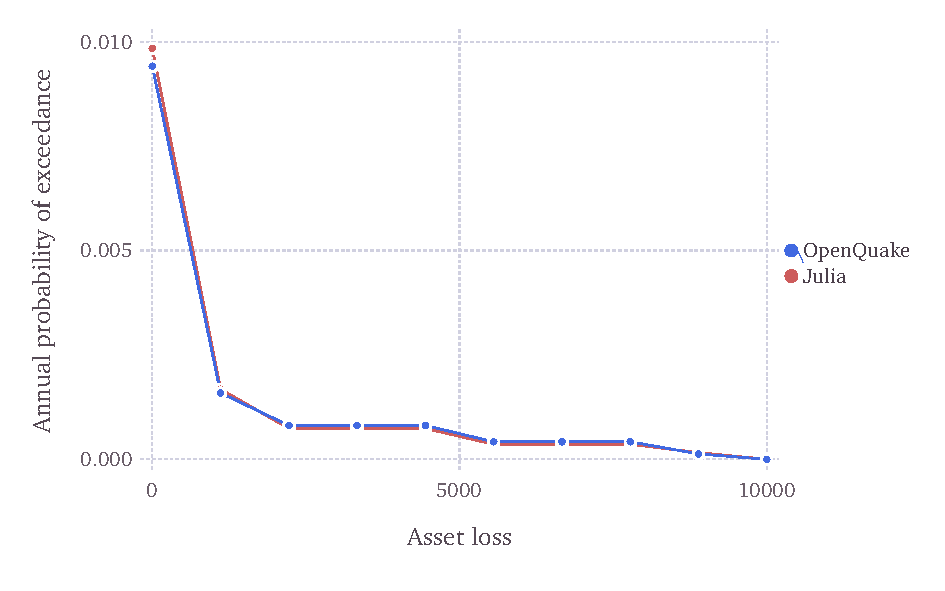
\includegraphics[width=12cm]{qareport/figures/fig-lc-ebr-1g}
\caption{Loss curve comparison for event based risk test case 1g}
\label{fig:lc-ebr-1g}
\end{figure}

The area under the annual loss exceedance curve gives the average annual loss.